\section{Feasibility of extrapolating links by paths}
\label{sec:ideas}

Our ultimate goal is to predict available bandwidth between two hosts by combining the 
end-to-end measurements from multiple video viewers and the
 routing information supplied by the routing engine. 


At first glance, it may appear that we need to  first extrapolate the available
bandwidth on {\em every link} in the network to predict the performance between
an arbitrary pair of  hosts.  However, in reality, it is sufficient to know
which link on the path between the two hosts is the {\em bottleneck} link and
focus only on estimating the available bandwidth of the bottleneck link.
Therefore, instead of an ``atlas'' where every link is annotated with its
available bandwidth, it suffices to have a  ``congestion map'' where only
bottleneck links are annotated with available bandwidth (generating congestion map using packet-level techniques has been studied in~\cite{dinu2011inferring}).  


 Having thus reformulated our problem, there are three conceptual steps in converting the end-to-end measurements to
the available bandwidth on the observed set of bottleneck links (i.e., to be determined) to create this
 intermediary step of a ``real-time congestion map''. Given 
 this congestion map, we can simply predict the minimum 
across all observed bottlenecks on a given end-to-end path   as the available bandwidth for that path.
 (Note that  a link may be a bottleneck for some path but it need not be the minimal bottleneck 
 for a different path.)


\begin{packeditemize}

	\item First, the  measurement from each video session is associated with the server and client IP (or AS depending on how much information the underlying streaming protocols provide). 

	\item Second, the client-server IP pairs are then mapped to link-level paths via routing information provided by other services (e.g., iPlane).

	\item Finally, we use an extrapolation algorithm to infer available bandwidth of all bottleneck links to generate a congestion map. In addition, the congestion map also include the information that all links along the path have at least the available bandwidth of the bottleneck link.

\end{packeditemize}


\begin{figure}[h!]
\begin{center}
%\includegraphics[]{p1_2Fig.ps}
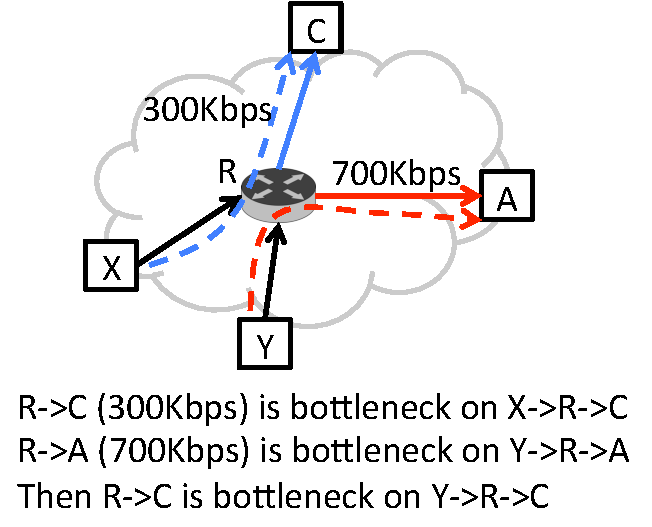
\includegraphics[scale=0.5] {figures/congestion_map.pdf}
\vspace{-0.4cm}
\caption{Example of congestion map. The available bandwidth between Y and C is calculated based on the congestion map -- Link YC has larger bandwidth than RA which is above RC, therefore, RC is bottleneck and available bandwidth of path Y to C is 300Kbps.}
\label{fig:idea:example}
\end{center}
\end{figure}

The key technique to identify bottleneck links for paths, called ``bottleneck
inference'', exploits the power of large number of overlapping paths,
and annotated the available bandwidth of the bottleneck link with the available
bandwidth of the path.  When given the path between two IP addresses, we
compare the available bandwidth of every link along it to identify the bottleneck link
with the lowest available bandwidth, and output that as the predicted available
bandwidth between the two IP addresses. Figure~\ref{fig:idea:example} shows how congestion map is used to identify bottleneck link and available bandwidth between two hosts.

%We now focus on the bottleneck
%inference technique. 
%We will use real topology and different traffic patterns to
%test its accuracy in identifying the bottlenecks and its coverage in predicting the
%available bandwidth for any two hosts as well. 
%\vyas{this only obtains bandwidth for the bottlenck links -- what about
%others}


\subsection{Bottleneck inference}
The basic idea of bottleneck inference algorithm is to rank the IP-level links
along the routing path of each session by the likelihood for it to be the bottleneck
link, and the likelihood is called {\it Bottleneck Score} (similar to ~\cite{agarwal2010webprofiler}). Note that only using this technique, we
cannot pinpoint which link is the bottleneck. Instead, this technique
enables to identify the link that is most likely to be the bottleneck
(i.e., with highest Bottleneck Score). 

The algorithm is based on two assumptions:
\begin{packeditemize}
	\item {\bf A1:} The available bandwidth of a path is identical to that of the bottleneck link, and 
	\item {\bf A2:} (Fair sharing) All paths sharing the same bottleneck link should receive at most the available bandwidth on the link.
\end{packeditemize}
Consequently, we have the following statements: ``{\it Given two paths $P,P'$ such that $P$ shares a link $L$ with $P'$, if $P'$ has a significantly higher bandwidth than $P$, then the bottleneck link of $P$ should not be $L$}''. The rationale is that if otherwise, $P$ is bottlenecked by link $L$, $P'$ should get at most the available bandwidth of $L$ ({\bf A2}) which is identical to the bandwidth seen by $P$ ({\bf A1}). However, this is contradict to the assumption. 
More realistically, taking into account other  parameters (e.g., round trip time, slow start time), the bandwidth $P'$ sees could be a bit different from what $P$ sees. So we only consider cases where $P'$ has bandwidth significantly higher (e.g., 50\% higher) than $P$. For example, in Figure~\ref{fig:idea:example}, since path from  $B$ to $D$ (10Mbps) has significantly higher bandwidth than from $A$ to $C$ (100Kbps), their overlapping link between $E$ and $F$ should not be the bottleneck of path from $A$ to $C$.

\begin{figure}[h]
\begin{center}
%\includegraphics[]{p1_2Fig.ps}
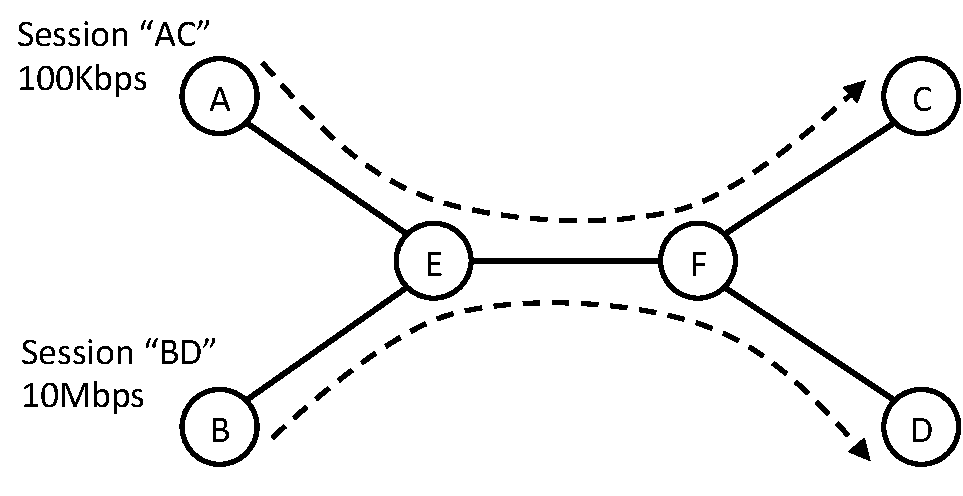
\includegraphics[scale=0.4] {figures/bottleneckExample.pdf}
\vspace{-0.5cm}
\caption{Simple example of bottleneck inference algorithm.}
\label{fig:idea:example}
\end{center}
\end{figure}

Based on this intuition, we calculate a Bottleneck Score for each link along a path that indicates how likely the link is to be a bottleneck as follows. Suppose that each path $P$ is a set of links along it, and for each link $L$ on path $P$, its Bottleneck Score is:
\begin{align*}
&BottleneckScore(L)\\
&=1-Pr\{BW(P') > 150\%\cdot BW(P) | L \in P \cap P'\}\\
&=1-\frac{|\{P'|\{BW(P') > 150\%\cdot BW(P), L \in P \cap P'\}|}{|\{P'|L \in P \cap P'\}|}
\end{align*}

Intuitively, the higher the Bottleneck Score is, the less the fraction of other paths indicating the link not being a bottleneck is, and thus in other words, the more likely the link is the bottleneck. The technique will return the links with the highest score. 
One thing needs to note is that if a link is not shared with other path (i.e., $\{P'|L\in P\cap P'\}=\emptyset$), the Bottleneck Score will become meaningless. This is usually caused by last mile links that only connect to a few users.
To avoid this problem, we aggregage client and server IP into /24 blocks, and predict the bottleneck along the path between two IP blocks. 


%We note that bottleneck link identification via path correlation has been studied before (e.g., \cite{agarwal2010webprofiler})


%% VS: either flesh this related work or dont say anything
%To rule out p
%ossible bottleneck link by correlating paths is not first proposed -- \cite{} has mentioned the same idea and \cite{} used path comparison to find system bottleneck in other scenarios. However, our contribution lies in ...

\begin{figure}[h]
\begin{center}
%\includegraphics[]{p1_2Fig.ps}
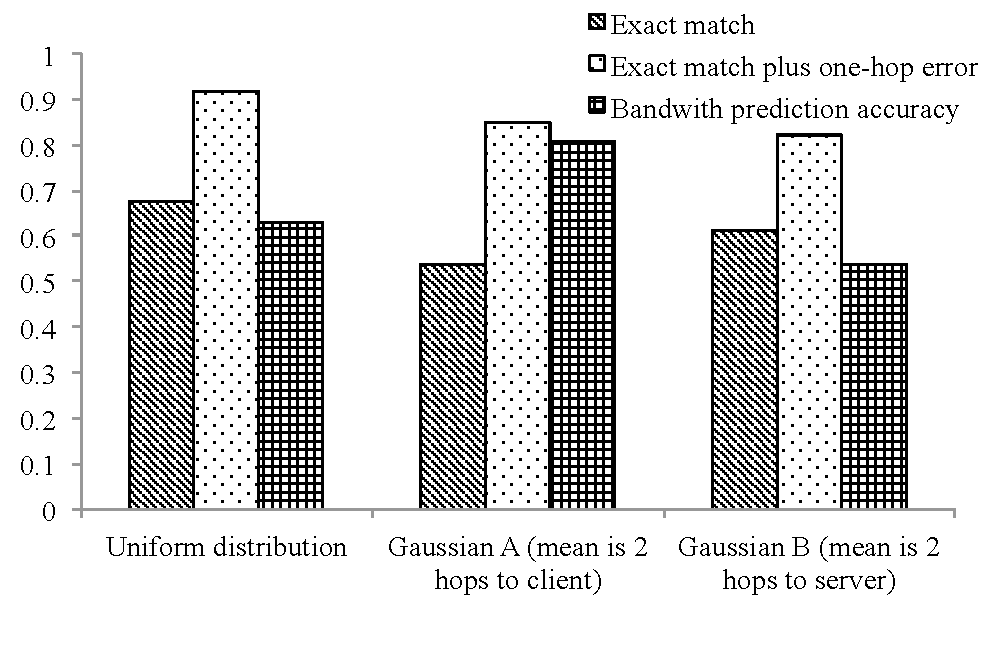
\includegraphics[scale=0.4] {figures/bottle-sim-bar-w-prediction.pdf}
\vspace{-0.9cm}
\caption{Simulation-based validation for bottleneck inference technique.}
\label{fig:cdn-criticalAttributeSets}
\end{center}
\end{figure}

\subsection{Simulation-based validation}
We now use a data-driven simulation to validate the proposed bottleneck
inference technique. The goal of the simulation is
to test the feasibility of bottleneck inference -- (i) how accurate it is to identify
bottleneck links in a real topology and various bottleneck distribution, and (ii) how accurate it is to use the identified bottlenecks to predict available bandwidth of any two hosts.

To this end, we use client requests in our own dataset and the path obtained
from iPlane to generate a real network topology of links that have been probed
by video sessions. We then randomly generate sessions between client and
servers by three bottleneck distributions -- uniformly
distribution through the network, skewed distribution such that bottlenecks are
closer to clients, and that bottlenecks are closer to
servers. To control the location of bottleneck for each session, we adjust the
volume of background traffic on each link. Finally, we run the bottleneck inference algorithm 
to localize the bottleneck links based on bandwidth seen by edge users and compare it with the ground truth.
Figure~\ref{fig:cdn-criticalAttributeSets} present the result under three bottleneck distributions. Each of them has run for
30 times and we show the average value. 

The first two bars show the bottleneck identification accuracy -- it is consistent that more than 80\% of the identified bottlenecks
are no more than 1 hop from the real bottlenecks. This error is tolerable in the hope
that one hop will not significantly change the location of the bottleneck
links. 
The last bar shows the bandwidth estimation accuracy -- we use the obtained congestion map to predict the available bandwidth between all pairs of edge users and compare it with the ground truth. It shows the accuracy (with less than 10\% error) also achieves as high as 80\%.


In summary, we find that by correlating views from multiple concurrent video flows, we are able to quite accurately locate bottleneck links, and based on these revealed bottleneck links (i.e., congestion map), the available bandwidth between any two hosts can be predicted with descent accuracy even with a simple unoptimized heuristic approach. We believe that we can further improve this with better estimation/laerning techniqies.
